\documentclass{beamer}
\usepackage{proof}
\usepackage{listings}
\usepackage{amsmath}
\usepackage{tikz}
\usetheme{Boadilla}
\title[Points-to Analysis using BDDs]{Points-to Analysis using BDDs}
\date{March 13, 2012}

\author[Marc Berndl et al.]{Marc Berndl, Ond\v{r}ej Lhot\'{a}k, Fend Qian, Laurie Hendren and Navindra Umanee \nocite{Berndl::PointsToBDDs}}
\begin{document}

\AtBeginSection[]
{
    \begin{frame}{Table of Contents}
        \tableofcontents[currentsection]
    \end{frame}
}

\begin{frame}
\titlepage
\begin{center}
Presented by Ismail Badawi
\end{center}
\end{frame}

\begin{frame}
\tableofcontents
\end{frame}

\section{Points-to analysis refresher}
\begin{frame}{Points-to analysis}
Goal: to determine the possible runtime values of a pointer. 

This is useful because it helps us to better approximate what is being
referenced or modified, which is generally important information that a
lot of analyses or optimizations depend on.
\end{frame}

\begin{frame}{Points-to analysis in Java} 
The analysis we're going to see is for Java. Features of note:
    \begin{itemize}
        \item Call-by-value (but those values might be references) 
        \item All allocation is dynamic (i.e. via {\tt new}) 
        \item No address-of operator 
        \item No multilevel pointers 
        \item No pointer arithmetic
    \end{itemize}
\end{frame}

\begin{frame}{Basics}
\nocite{Hind::PointerAnalysis}
\begin{itemize}
\item Compute a \emph{points-to relation} $S$, mapping identifiers to
      allocation sites. $(a, A) \in S$ if variable $a$ could potentially
      point to $A$.
\item This is a well-known problem, which has been worked on for a long
time; there are many ways to classify approaches taken:
    \begin{itemize}
      \item flow sensitive vs.  flow insensitive
        \begin{itemize}
        \item subset-based vs. equality-based
        \end{itemize}
    \end{itemize}
\end{itemize}
\end{frame}

\begin{frame}{Flow sensitivity}
Does the analysis model control flow at all?
\begin{itemize}
\item Flow-sensitive: essentially just dataflow analysis
    \begin{itemize}
    \item More accurate results for each program point
    \item Can get \emph{really} complicated...
    \item Tends to be quite slow
    \end{itemize}
\item Flow-insensitive: constraint satisfaction
  \begin{itemize}
    \item Every allocation, assignment, etc. potentially affects the
          points-to relation
    \item Gather them all up in a big list, and propagate points-to
          relationships until a fixed point is reached
    \item Less accurate, one approximation for the whole program
    \item Faster!
  \end{itemize}
\end{itemize}
\end{frame}

\begin{frame}{Equality based vs. subset based}
Flow-insensitive analyses can be further split into equality based and
subset based analyses.
\begin{itemize}
\item Equality based: assignments are bidirectional
  \begin{itemize}
  \item {\tt a = b;}? Now $a$ and $b$ have the same points-to sets
  \end{itemize}
\item Subset based: assignments are unidirectional
  \begin{itemize}
  \item {\tt a = b;}? Now $a$ can point to anything $b$ can point to, but not vice versa
  \end{itemize}
\end{itemize}
Obviously subset-based analyses are more accurate, but they are also more
challenging to implement efficiently.
\end{frame}

\begin{frame}{Using BDDs}
The analysis we're going to see today is flow-insensitive, and subset-based.

\end{frame}

\begin{frame}{Simple example}
\begin{table}\small
\begin{tabular}{l l}
\\
{\tt A: a = new O();} & \onslide<2->{$\{(a, A)\}$} \\
{\tt B: b = new O();} & \onslide<2->{$\{(a, A), (b, B)\}$} \\
{\tt C: c = new O();} & \onslide<2->{$\{(a, A), (b, B), (c, C)\}$} \\
{\tt a = b;} & \only<3>{$\{(a, A), {\color{green} (a, B)}, (b, B), (c, C)\}$}\onslide<4->{$\{(a, A), (a, B), (b, B), (c, C)\}$} \\
{\tt b = a;} & \only<4>{$\{(a, A), (a, B), {\color{green} (b, A)}, (b, B), (c, C)\}$}\onslide<5->{$\{(a, A), (a, B), (b, A), (b, B), (c, C)\}$} \\
{\tt c = b;} & \only<5>{$\{(a, A), (a, B), (b, A), (b, B), (c, A), {\color{green} (c, B)}, {\color{green} (c, C)}\}$}
\end{tabular}
\end{table}
\end{frame}         

\begin{frame}{What did we learn?}
Let $pt(x)$ (the \emph{points-to set} of $x$) denote the set of allocation
sites $x$ could point to. Then we have:
$$ pt(a) = \{A, B\} \qquad pt(b) = \{A, B\} \qquad pt(c) = \{A, B, C\} $$
\pause
Notice:
\begin{itemize}
\item There are many points-to sets
\item Points-to sets can get quite big
\item Points-to sets are often equal or almost equal
\end{itemize}
Goal: an efficient, compact representation for points-to sets.
\end{frame}

\section{Binary decision diagrams}
\nocite{Bryant::BDDs}
\begin{frame}{Binary decision diagrams}
\begin{itemize}
\item A binary decision diagram (BDD) is a directed acyclic graph.
\begin{itemize}
\item It has a root node.
\item It has two terminal (leaf) nodes, \fbox{0} and \fbox{1}.
\item Every non-leaf node has a $0$-successor and a $1$-successor.
\end{itemize}
\end{itemize}

A path from the root to a terminal node corresponds to a binary string of
length $n$, where $n$ is the height of the BDD.
\end{frame}

\begin{frame}{Interpretation}
Two ways of looking at a BDD $S$
\begin{itemize}
\item As a \emph{set of binary strings}.
  \begin{itemize}
    \item $b_1b_2 \dots b_n \in S$ iff the path $b_1, b_2, \dots, b_n$ ends at \fbox{1}
  \end{itemize}
\item As a \emph{binary function}
    \begin{itemize}
    \item $S: \{0, 1\}^n \rightarrow \{0, 1\}$
    \item $S(b_1, b_2, \dots, b_n) = 1$ iff the path $b_1, b_2, \dots, b_n$ ends at \fbox{1}
    \item Can view as the \emph{characteristic function} of a set $S$, i.e.
    $$ S(b_1, ..., b_n) = \chi_S(b_1...b_n) = \begin{cases}
      1 & \text{if } b_1...b_n \in S \\
      0 & \text{if } b_1...b_n \not \in S
    \end{cases}$$
    \end{itemize}
\end{itemize}
\end{frame}

\tikzstyle{int} = [circle, draw]
\tikzstyle{term} = [rectangle, draw]
                  
\begin{frame}{BDD Example}
\begin{columns}
\column{2.5in}
\begin{tikzpicture}
    \node[int] (start) at (5, 10) {};
    \node[int] (0) at (3, 9) {};
    \node[int] (1) at (7, 9) {};
    \node[int] (00) at (2, 8) {};
    \node[int] (01) at (4, 8) {};
    \node[int] (10) at (6, 8) {};
    \node[int] (11) at (8, 8) {};
    \node[term] (ZERO) at (4, 7) {0};
    \node[term] (ONE) at (6, 7) {1};
    \foreach \from/\to in {start/1, 0/01, 1/11, 00/ZERO, 01/ZERO, 10/ONE, 11/ONE}
        \draw[->] (\from) -- (\to);
    \foreach \from/\to in {start/0, 0/00, 1/10, 00/ONE, 01/ONE, 10/ZERO, 11/ZERO}
        \draw[->, densely dotted] (\from) -- (\to);
\end{tikzpicture}
\column{1.5in}
This BDD represents the set $\{000, 010, 101, 111\}$.
\end{columns}
\end{frame}

\begin{frame}{Reducing BDDs}
\begin{columns}
\column{2.5in}
\begin{tikzpicture}
    \node[int] (start) at (5, 10) {};
    \node[int] (0) at (3, 9) {};
    \node[int] (1) at (7, 9) {};
    \node[int] (00) at (2, 8) {};
    \node[int] (01) at (4, 8) {};
    \node[int] (10) at (6, 8) {};
    \node[int] (11) at (8, 8) {};
    \node[term] (ZERO) at (4, 7) {0};
    \node[term] (ONE) at (6, 7) {1};
    \foreach \from/\to in {start/1, 0/01, 1/11, 00/ZERO, 01/ZERO, 10/ONE, 11/ONE}
        \draw[->] (\from) -- (\to);
    \foreach \from/\to in {start/0, 0/00, 1/10, 00/ONE, 01/ONE, 10/ZERO, 11/ZERO}
        \draw[->, densely dotted] (\from) -- (\to);
\end{tikzpicture}
\column{1.5in}                       
\only<1>{Actually this is more like a binary decision tree. We can do better than this!}
\onslide<2->{Can merge nodes with identical successors at the same level...}
\end{columns}
\end{frame}

\begin{frame}{Reduced BDD (1)}
\begin{columns}[c]
\column{1.5in}
\begin{tikzpicture}
    \node[int] (start) at (5, 10) {};
    \node[int] (0) at (3, 9) {};
    \node[int] (1) at (7, 9) {};
    \node[int] (0x) at (3, 8) {};
    \node[int] (1x) at (7, 8) {};
    \node[term] (ZERO) at (4, 7) {0};
    \node[term] (ONE) at (6, 7) {1};
    \draw[->, densely dotted] (start) -- (0);
    \draw[->] (start) -- (1);
    \draw[->, densely dotted] (0) to [bend right] (0x);
    \draw[->] (0) to [bend left] (0x);
    \draw[->, densely dotted] (1) to [bend right] (1x);
    \draw[->] (1) to [bend left] (1x);
    \draw[->, densely dotted] (0x) -- (ONE);
    \draw[->] (0x) -- (ZERO);
    \draw[->, densely dotted] (1x) -- (ZERO);
    \draw[->] (1x) -- (ONE);
\end{tikzpicture}
\column{1.5in}
\pause
Can remove nodes where both successors are the same...
\end{columns}
\end{frame}

\begin{frame}{Reduced BDD (2)}
\begin{columns}[c]
\column{1.5in}
\begin{tikzpicture}
    \node[int] (start) at (5, 10) {};
    \node[int] (0x) at (3, 8) {};
    \node[int] (1x) at (7, 8) {};
    \node[term] (ZERO) at (4, 7) {0};
    \node[term] (ONE) at (6, 7) {1};
    \draw[->, densely dotted] (start) -- (0x);
    \draw[->] (start) -- (1x);
    \draw[->, densely dotted] (0x) -- (ONE);
    \draw[->] (0x) -- (ZERO);
    \draw[->, densely dotted] (1x) -- (ZERO);
    \draw[->] (1x) -- (ONE);
\end{tikzpicture}              
\column{1.5in}
This BDD represents the same set, and is completely reduced.

For a fixed ordering of the bits, reduced BDDs are unique.
\end{columns}
\end{frame}

\begin{frame}{Ordered BDDs}
\begin{itemize}
\item The order in which we test the bits is not important (as long as it's
consistent).
\item But the order of the bits can affect the size of the BDD. Suppose we
want to represent the set $\{000, 010, 100, 110\}$. If test the bits in
reverse order, we get this BDD: 

\begin{tikzpicture}
\node[int] (start) at (1, 1) {};
\node[term] (ZERO) at (0, 0) {0};
\node[term] (ONE) at (2, 0) {1};
\draw[->, densely dotted] (start) -- (ONE);
\draw[->] (start) -- (ZERO);
\end{tikzpicture}
\end{itemize}
\end{frame}

\begin{frame}{Remark}
The size of a BDD is not correlated with the size of the set it represents.
Contrived example: assume we have n bits. Then this BDD:
$$\fbox{0}$$
has one node, and represents the empty set. This BDD:
$$\fbox{1}$$
also has one node, but represents a set with $2^n$ elements.

In fact BDDs are often quite small relative to their set...
\end{frame}

\begin{frame}{Operations on BDDs}
\begin{itemize}
\item As it turns out, most of the interesting operations on BDDs run in
time linear in the number of nodes (not the size of the set)!
\item Given two BDDs $G_1$ and $G_2$, we can apply any binary operation 
in time $O(|G_1||G_2|)$. 
\item {\tt apply: (bit -> bit -> bit) -> bdd -> bdd -> bdd} 
    \begin{itemize}
        \item $\cup$: {\tt (apply or)} 
        \item $\cap$: {\tt (apply and)} 
        \item $\setminus$: {\tt (apply ($\lambda$ x. $\lambda$ y. => x and not y))}
    \end{itemize}
\end{itemize}
\end{frame}

\begin{frame}{Encoding relations}
\begin{itemize}
\item How do we use BDDs to represent relations? 
\item Back to our simple example, we have 
$$V = \{a, b, c\} \qquad H = \{A, B, C\}$$ 
$$pt \subseteq V \times H = \{(a, A), (a, B), (b, A), (b, B), (c, A), (c, B), (c, C)\}.$$
\item Assign to each set a \emph{variable domain}, a subset of the bits in a
binary string, and enumerate all the elements.
\begin{itemize}
    \item $a = 00, b = 01, c = 10, A = 00, B = 01, C = 10$
    \item $pt = \{0000, 0001, 0100, 0101, 1000, 1001, 1010\}$
    \item Each $p \in pt$ has the form $v_1v_2h_1h_2$
\end{itemize}
\end{itemize}
\end{frame}

\begin{frame}{More operations}
\begin{itemize}
\item Replace
  \begin{itemize}
    \item Given a BDD, create a new BDD where information that was stored
    in a certain domain is moved to another domain
  \end{itemize}
\item Existential quantification
  \begin{itemize}
    \item Given $P \subseteq V \times H$, existential quantification over $H$ computes
    $$ \{ v \in V \mid \exists h \in H. (v, h) \in P \} $$
    \end{itemize}
\item Relational product
  \begin{itemize}
    \item Combines existential quantification and set intersection
    \item $relprod(X, Y, V1)$ computes
    $$\{(x, y) \mid \exists v \in V1 . (v, x) \in X \wedge (v, y) \in Y)\}$$
  \end{itemize}
\end{itemize}
We will see how these are useful later.
\end{frame}

\section{Points-to relationships using BDDs}
\begin{frame}{Four kinds of constraints}
    \begin{itemize}
        \item Allocation
        $$ a: l := {\tt new} \, C \Longrightarrow o_a \in pt(l) $$
        \item Assignment
        $$ l_2 := l_1 \Longrightarrow l_1 \rightarrow l_2 $$
        \item Field store
        $$ q.f := l \Longrightarrow l \rightarrow q.f $$
        \item Field load
        $$ l := p.f \Longrightarrow p.f \rightarrow l $$
    \end{itemize}
\end{frame}

\begin{frame}{Variable domains}
\begin{itemize}
\item $V1$ and $V2$, variables of pointer type
  \begin{itemize} \item Need two to represent assignments \end{itemize}
\item $FD$, the set of field signatures
\item $H1$ and $H2$, allocation sites
  \begin{itemize} \item Need two, together with $FD$, to represent e.g.
  $o_2 \in pt(o_1.f)$ \end{itemize}
\end{itemize}
\end{frame}

\begin{frame}{BDDs used}
\begin{itemize}
\item $pointsTo \subseteq V1 \times H1$
  \begin{itemize} \item Points-to sets for variables, $o \in pt(l)$ \end{itemize}
\item $fieldPt \subseteq (H1 \times FD) \times H2$
  \begin{itemize} \item Points-to sets for fields of heap objects, $o_2 \in pt(o_1.f)$ \end{itemize}
\item $edgeSet \subseteq V1 \times V2$ 
  \begin{itemize} \item Simple assignments, $l_1 \rightarrow l_2$ \end{itemize}
\item $stores \subseteq V1 \times (V2 \times FD)$
  \begin{itemize} \item Field stores, $l_1 \rightarrow l_2.f$ \end{itemize}
\item $loads \subseteq (V1 \times FD) \times V2$
  \begin{itemize} \item Field loads, $l_1.f \rightarrow l_2$ \end{itemize}
\item $typeFilter \subseteq V1 \times H1$
  \begin{itemize} \item Used to restrict points-to sets based on declared types \end{itemize}
\end{itemize}
\end{frame}

\begin{frame}{Inference rules}
\begin{itemize}
\item Assignment \\
$$
\infer{o \in pt(l_2)}{l_1 \rightarrow l_2 & o \in pt(l_1)}
$$ 
\item Field store \\
$$
\infer{o_2 \in pt(o_1.f)}{o_2 \in pt(l) & l \rightarrow q.f & o_1 \in pt(q)}
$$
\item Field load \\
$$
\infer{o_2 \in pt(l)}{p.f \rightarrow l & o_1 \in pt(p) & o_2 \in pt(o_1.f)}
$$
\end{itemize}
Keep applying these rules until the points-to sets stop changing.
\end{frame}  

\lstdefinestyle{highlight} {
    keywordstyle=\color{red},
}
\lstdefinestyle{base}{
    basicstyle=\tiny\ttfamily\color{black!40},
    morekeywords={repeat,until,intersect,union,relprod,replace},
    moredelim=**[is][\only<+>{\color{black}\lstset{style=highlight}}]{@}{@},
}

\begin{frame}[fragile]{The algorithm}
\begin{lstlisting}[style=base]
repeat
  repeat
    @/* --- rule 1 --- */
    newPt1:[V2xH1] = relprod(edgeSet:[V1xV2], pointsTo:[V1xH1], V1);
    newPt2:[V1xH1] = replace(newPt1:[V2xH1], V2ToV1);@

    /* --- apply type filtering and merge into pointsTo relation --- */
    newPt3:[V1xH1] = newPt2:[V1xH1] intersect typeFilter:[V1xH1];
    pointsTo:[V1xH1] = pointsTo[V1xH1] union newPt3:[V1xH1];
  until pointsTo does not change

  /* --- rule 2 --- */
  tmpRel1:[(V2xFD)xH1] = relprod(stores[V1x(V2xFD)], pointsTo:[V1xH1], V1);
  tmpRel2:[(V1xFD)xH2] = replace(tmpRel1:[(V2xFD)xH1], V2ToV1 & H1ToH2);
  fieldPt:[(H1xFD)xH2] = relprod(tmpRel2:[(V1xFD)xH2], pointsTo:[V1xH1], V1);

  /* --- rule 3 --- */
  tmpRel3:[(H1xFD)xV2)] = relprod(loads:[(V1xFD)xV2], pointsTo:[V1xH1], V1);
  newPt4:[V2xH2] = relprod(tmpRel3:[(H1xFD)xV2], fieldPt:[(H1xFD)xH2], H1xFD);
  newPt5:[V1xH1] = replace(newPt4:[V2xH2], V2ToV1 & H2ToH1);

  /* --- apply type filtering and merge into pointsTo relation --- */
  newPt6:[V1xH1] = newPt5:[V1xH1] intersect typeFilter:[V1xH1];
  pointsTo:[V1xH1] = pointsTo:[V1xH1] union newPt6:[V1xH1];
until pointsTo does not change
\end{lstlisting}
\end{frame}

\begin{frame}{Applying rule 1}
Recall:
\begin{align*}
edgeSet &= \{ (l_1, l_2) \in V1 \times V2 \mid l_1 \rightarrow l_2 \} \\
pointsTo &= \{ (l, o) \in V1 \times H1 \mid o \in pt(l) \} \\
relprod(X, Y, V1) &= \{(x, y) \mid \exists v \in V1.(v, x) \in X \wedge (v, y) \in Y\}
\end{align*}
So...
\begin{align*}
&relprod(edgeSet, pointsTo, V1) \\&= \{ (l_2, o) \mid \exists l_1 \in V1. (l_1, l_2) \in edgeSet \wedge (l_1, o) \in pointsTo \} \\
&= \{ (l_2, o) \mid \exists l_1. l_1 \rightarrow l_2 \wedge o \in pt(l_1) \}
\end{align*}
This is exactly the rule for simple assignments!
\end{frame}

\begin{frame}[fragile]{The algorithm}
\begin{lstlisting}[style=base]
repeat
  repeat
    /* --- rule 1 --- */
    newPt1:[V2xH1] = relprod(edgeSet:[V1xV2], pointsTo:[V1xH1], V1);
    newPt2:[V1xH1] = replace(newPt1:[V2xH1], V2ToV1);

    /* --- apply type filtering and merge into pointsTo relation --- */
    newPt3:[V1xH1] = newPt2:[V1xH1] intersect typeFilter:[V1xH1];
    pointsTo:[V1xH1] = pointsTo[V1xH1] union newPt3:[V1xH1];
  until pointsTo does not change

  @/* --- rule 2 --- */
  tmpRel1:[(V2xFD)xH1] = relprod(stores[V1x(V2xFD)], pointsTo:[V1xH1], V1);
  tmpRel2:[(V1xFD)xH2] = replace(tmpRel1:[(V2xFD)xH1], V2ToV1 & H1ToH2);
  fieldPt:[(H1xFD)xH2] = relprod(tmpRel2:[(V1xFD)xH2], pointsTo:[V1xH1], V1);@

  /* --- rule 3 --- */
  tmpRel3:[(H1xFD)xV2)] = relprod(loads:[(V1xFD)xV2], pointsTo:[V1xH1], V1);
  newPt4:[V2xH2] = relprod(tmpRel3:[(H1xFD)xV2], fieldPt:[(H1xFD)xH2], H1xFD);
  newPt5:[V1xH1] = replace(newPt4:[V2xH2], V2ToV1 & H2ToH1);

  /* --- apply type filtering and merge into pointsTo relation --- */
  newPt6:[V1xH1] = newPt5:[V1xH1] intersect typeFilter:[V1xH1];
  pointsTo:[V1xH1] = pointsTo:[V1xH1] union newPt6:[V1xH1];
until pointsTo does not change
\end{lstlisting}
\end{frame} 

\begin{frame}{Applying rule 2}
\begin{align*}
stores &= \{ (l_1, (l_2, f)) \in V1 \times (V2 \times FD) \mid l_1 \rightarrow l_2.f \} \\
pointsTo &= \{ (l, o) \in V1 \times H1 \mid o \in pt(l) \} \\
relprod(X, Y, V1) &= \{(x, y) \mid \exists v \in V1.(v, x) \in X \wedge (v, y) \in Y\} \\
\\
tmpRel &= relprod(stores, pointsTo, V1) \\
       &= \{ (o_2, q.f) \mid \exists l. o_2 \in pt(l) \wedge l \rightarrow q.f \} \\
\end{align*}
So...
\begin{align*}
&relprod(tmpRel, pointsTo, V1) \\&= \{ (o_2, o_1.f) \mid \exists q (\exists l. o_2 \in pt(l) \wedge l \rightarrow q.f) \wedge o_1 \in pt(q) \}
\end{align*}
\end{frame}

\begin{frame}[fragile]{The algorithm}
\begin{lstlisting}[style=base]
repeat
  repeat
    /* --- rule 1 --- */
    newPt1:[V2xH1] = relprod(edgeSet:[V1xV2], pointsTo:[V1xH1], V1);
    newPt2:[V1xH1] = replace(newPt1:[V2xH1], V2ToV1);

    /* --- apply type filtering and merge into pointsTo relation --- */
    newPt3:[V1xH1] = newPt2:[V1xH1] intersect typeFilter:[V1xH1];
    pointsTo:[V1xH1] = pointsTo[V1xH1] union newPt3:[V1xH1];
  until pointsTo does not change

  /* --- rule 2 --- */
  tmpRel1:[(V2xFD)xH1] = relprod(stores[V1x(V2xFD)], pointsTo:[V1xH1], V1);
  tmpRel2:[(V1xFD)xH2] = replace(tmpRel1:[(V2xFD)xH1], V2ToV1 & H1ToH2);
  fieldPt:[(H1xFD)xH2] = relprod(tmpRel2:[(V1xFD)xH2], pointsTo:[V1xH1], V1);

  @/* --- rule 3 --- */
  tmpRel3:[(H1xFD)xV2)] = relprod(loads:[(V1xFD)xV2], pointsTo:[V1xH1], V1);
  newPt4:[V2xH2] = relprod(tmpRel3:[(H1xFD)xV2], fieldPt:[(H1xFD)xH2], H1xFD);
  newPt5:[V1xH1] = replace(newPt4:[V2xH2], V2ToV1 & H2ToH1);@

  /* --- apply type filtering and merge into pointsTo relation --- */
  newPt6:[V1xH1] = newPt5:[V1xH1] intersect typeFilter:[V1xH1];
  pointsTo:[V1xH1] = pointsTo:[V1xH1] union newPt6:[V1xH1];
until pointsTo does not change
\end{lstlisting}
\end{frame} 

\begin{frame}{How do we use this?}
We end up with a BDD $G$ that represents the points-to relation implicitly. How do we access this information?
\begin{itemize}
\item Could enumerate the solutions and construct a more explicit
representation
  \begin{itemize}
    \item Turns out this takes time $O(|G|M)$, where $M$ is the number of
    bits used to encode $G$
    \item The explicit representation could also be quite large!
  \end{itemize}
\item Could extract points-to sets of specific variables on demand
\item Could keep the BDD and use BDD operations for our queries
\end{itemize}
\end{frame}

\section{Results}
\begin{frame}{Performance}
Depends \emph{dramatically} on ordering of $V1, V2, FD, H1, H2$ \\
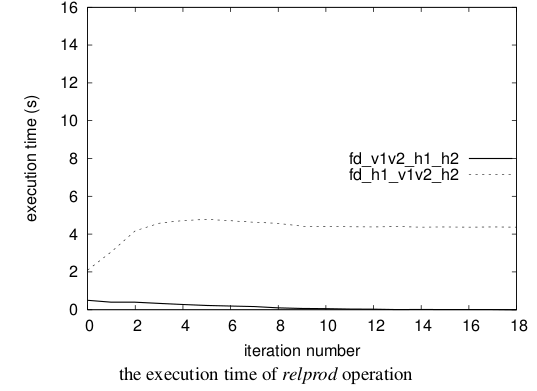
\includegraphics[scale=0.4]{domain-arrangement.png}
\end{frame}

\begin{frame}{Interleaving}
Can also choose whether to interleave domains or place them sequentially... \\
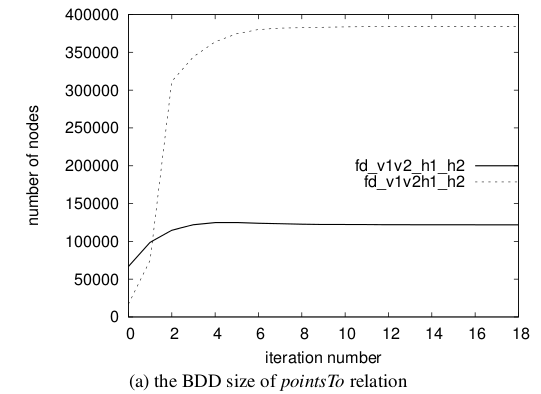
\includegraphics[scale=0.25]{interleaving-1.png} \qquad
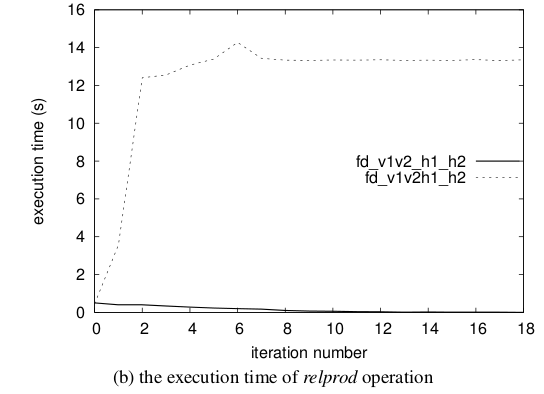
\includegraphics[scale=0.25]{interleaving-2.png}
\end{frame}

\begin{frame}{Good idea?}
\begin{itemize}
\item Compared to an efficient hand-coded solver based on SPARK, a previous
Sable group project
\item Performance is comparable, better for really big programs
\item Clear winner for memory usage!
\end{itemize}
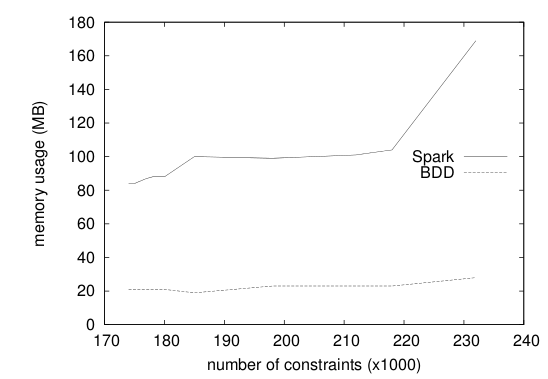
\includegraphics[scale=0.25]{performance.png}
\end{frame}

\section{Questions}
\begin{frame}{Short questions}
\begin{enumerate}
\item Some operations on BDDs can be done in constant time. One of them is
\emph{complementation}. Give a constant-time algorithm for complementing a
BDD. \\
\pause
Answer: Swap the two terminal nodes.
\pause
\item How would you handle function calls with a flow-insensitive approach
like this one? (There are many possible answers here.) \\
\pause
Answer: Function calls are modeled by constructing a call graph (using
class hierarchy analysis) and adding assignment edges where appropriate to
simulate parameter passing and return values.
\end{enumerate}
\end{frame}

\begin{frame}[fragile]{Assignment question}
Run the BDD points-to algorithm for our simple example from earlier. 
\begin{itemize}
\item Start by listing all the constraints.
\item Draw all relevant BDDs at every step. 
\item You don't need to show the details of how {\tt apply}, {\tt relprod}
or {\tt replace} work. If you want, you can figure out the resulting set of
strings manually, and from there determine what the BDD looks like. 
\item You should draw BDDs totally reduced, but there is no need to show 
the reduction process. 
\item You may use any variable ordering. 
\item You may ignore type filtering. 
\item You should be able to produce one BDD representing the entire 
points-to relation.
\end{itemize}
\end{frame}

\begin{frame}{References}
\bibliographystyle{plain}
{\footnotesize
\bibliography{bib}}
\end{frame}

\end{document}
